% =========================================================================
% EXPERIMENT 2 - PROBLEM 1: COLLEGE DATABASE DDL
% =========================================================================
\label{exp:ddl}
\label{exp:ddl_prob1}
\noindent
\begin{center}
    {\LARGE \textbf{DBMS LABORATORY PRACTICAL}}\\[0.25cm]
    \textbf{Practical No.:} 2 (Problem 1) \hfill \textbf{Date:} 06/10/2026 \hfill \textbf{Page No.:} \thepage
\end{center}
\vspace{-0.2cm}
\hrule
\vspace{0.35cm}

\subsection*{Question / Problem Statement}
Consider the database for a college. Design and implement the relational database schema using Data Definition Language (DDL) commands in MySQL:
\begin{enumerate}[noitemsep,topsep=2pt]
    \item[(i)] Create the database \texttt{college} and select it as the active database context.
    \item[(ii)] Create the following relational tables with their integrity constraints: \texttt{Department}, \texttt{Student}, \texttt{Faculty}, \texttt{Course}, \texttt{Register}, \texttt{Teaching}, and \texttt{Hostel}.
    \item[(iii)] Enforce primary key, foreign key, not null, unique, check, and default constraints.
    \item[(iv)] Display all tables in the database using \texttt{SHOW TABLES;}.
    \item[(v)] Describe the schema structure of all tables using \texttt{DESCRIBE}.
    \item[(vi)] Modify the \texttt{Student} table to add a new column \texttt{grade CHAR(2)} via \texttt{ALTER TABLE}.
\end{enumerate}

\subsection*{1. Database \& Table Creation with Integrity Constraints}

\subsubsection*{SQL Query}
\begin{lstlisting}[basicstyle=\ttfamily\footnotesize,caption={Creating college database and relational tables with integrity constraints}]
-- Create and select college database
CREATE DATABASE college;
USE college;

-- 1. Department table
CREATE TABLE Department (
    dno INT PRIMARY KEY,
    dname VARCHAR(50) NOT NULL UNIQUE
);

-- 2. Student table (referencing Department)
CREATE TABLE Student (
    sid INT PRIMARY KEY,
    sname VARCHAR(50) NOT NULL,
    sex CHAR(1) CHECK (sex IN ('M', 'F', 'O')),
    dob DATE NOT NULL,
    dno INT,
    FOREIGN KEY (dno) REFERENCES Department(dno)
);

-- 3. Faculty table (referencing Department)
CREATE TABLE Faculty (
    f_id INT PRIMARY KEY,
    fname VARCHAR(50) NOT NULL,
    designation VARCHAR(50) DEFAULT 'Assistant Professor',
    salary DECIMAL(10, 2) CHECK (salary > 0),
    dno INT,
    FOREIGN KEY (dno) REFERENCES Department(dno)
);

-- 4. Course table (referencing Department)
CREATE TABLE Course (
    cid INT PRIMARY KEY,
    cname VARCHAR(50) NOT NULL UNIQUE,
    credits INT CHECK (credits BETWEEN 1 AND 6),
    dno INT,
    FOREIGN KEY (dno) REFERENCES Department(dno)
);

-- 5. Register table (composite primary key and foreign keys)
CREATE TABLE Register (
    sid INT,
    cid INT,
    sem INT DEFAULT 1,
    PRIMARY KEY (sid, cid),
    FOREIGN KEY (sid) REFERENCES Student(sid),
    FOREIGN KEY (cid) REFERENCES Course(cid)
);

-- 6. Teaching table (composite primary key and foreign keys)
CREATE TABLE Teaching (
    f_id INT,
    cid INT,
    sem INT DEFAULT 1,
    PRIMARY KEY (f_id, cid),
    FOREIGN KEY (f_id) REFERENCES Faculty(f_id),
    FOREIGN KEY (cid) REFERENCES Course(cid)
);

-- 7. Hostel table
CREATE TABLE Hostel (
    hid INT PRIMARY KEY,
    hname VARCHAR(50) NOT NULL UNIQUE,
    seats INT DEFAULT 100 CHECK (seats > 0)
);
\end{lstlisting}

\vspace{0.2cm}

\subsection*{2. Schema Inspection \& Dynamic Alteration}

\subsubsection*{SQL Query}
\begin{lstlisting}[basicstyle=\ttfamily\footnotesize,caption={Displaying tables, inspecting schemas, and altering table structure}]
-- Display all created tables in college database
SHOW TABLES;

-- Inspect schema definitions and constraints
DESCRIBE Department;
DESCRIBE Student;
DESCRIBE Faculty;
DESCRIBE Course;
DESCRIBE Register;
DESCRIBE Teaching;
DESCRIBE Hostel;

-- Dynamically alter Student table to add grade column
ALTER TABLE Student ADD COLUMN grade CHAR(2);
\end{lstlisting}

\newpage

\subsection*{Output Screenshots}

\begin{figure}[H]
    \centering
    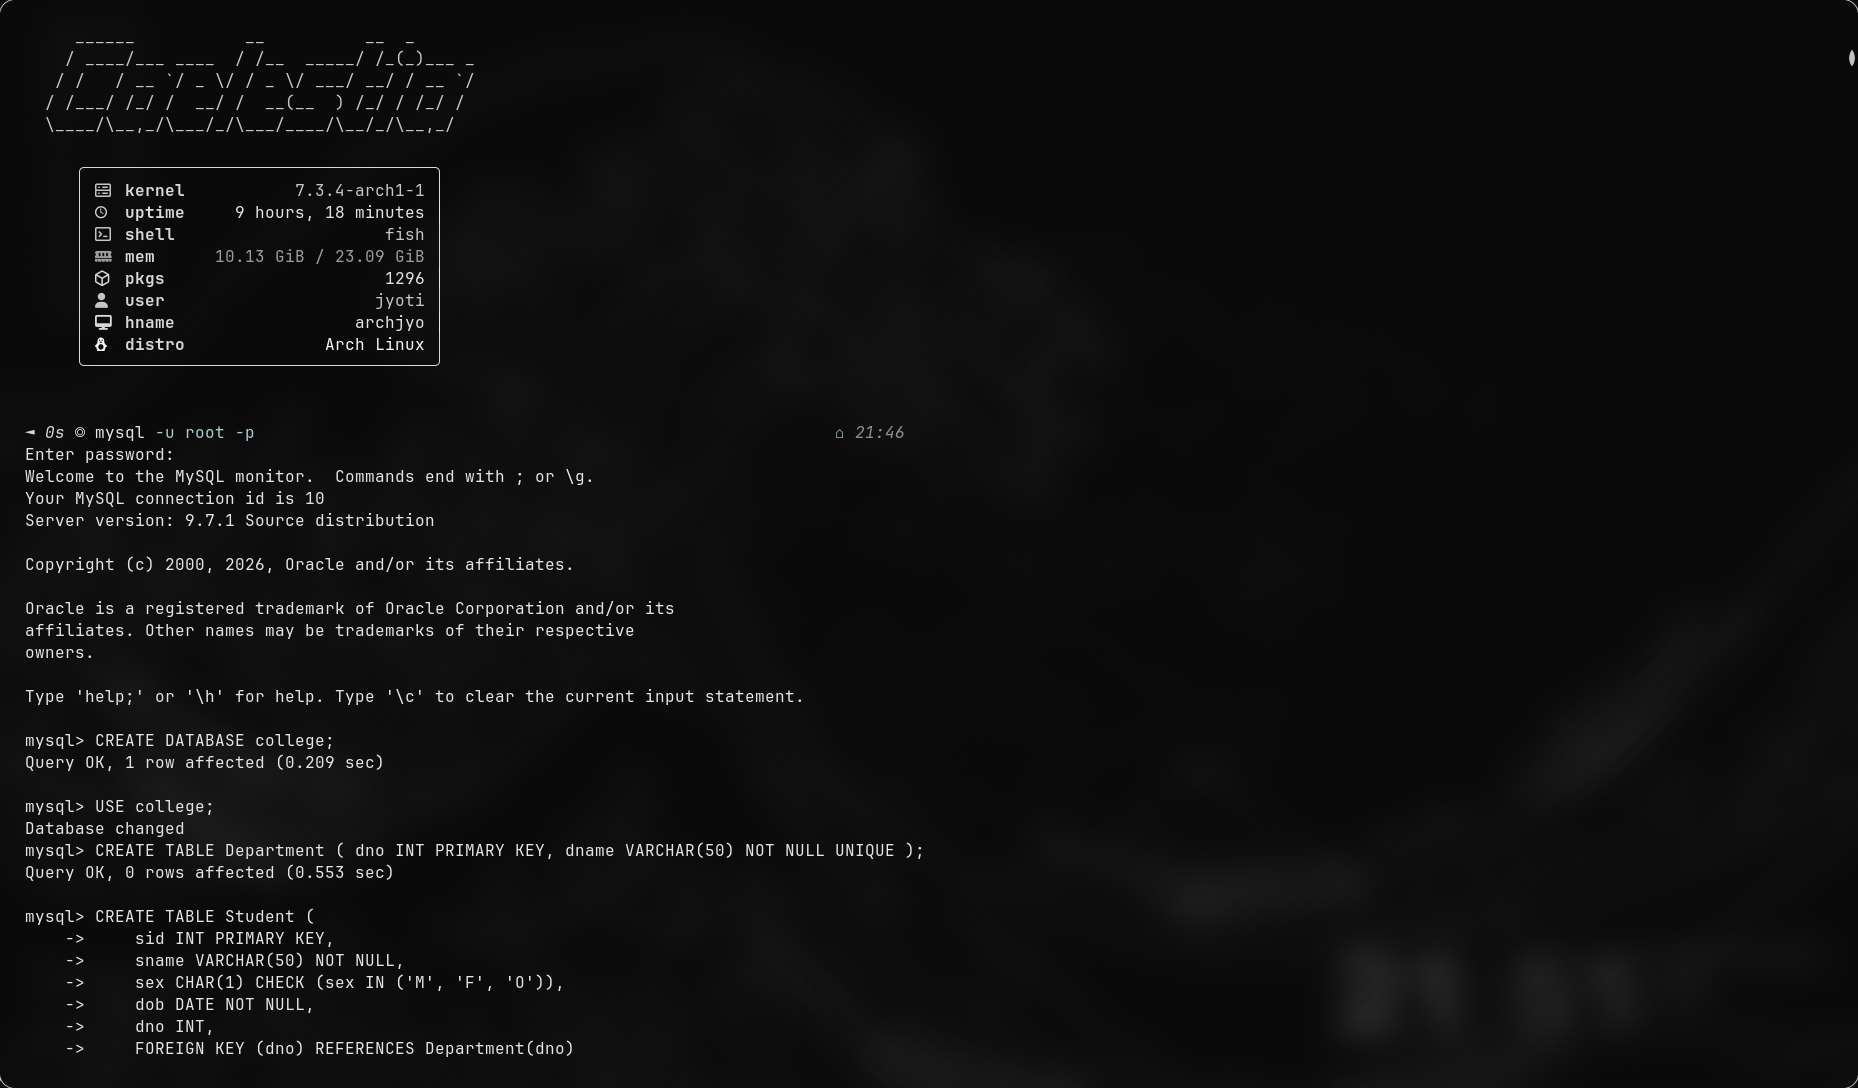
\includegraphics[width=0.92\linewidth,height=7.8cm,keepaspectratio]{Exp2-prob1-1.png}
    \caption{Database creation, active context selection, and Department/Student table creation.}
    \label{fig:exp2_create1}
\end{figure}

\vspace{0.2cm}

\begin{figure}[H]
    \centering
    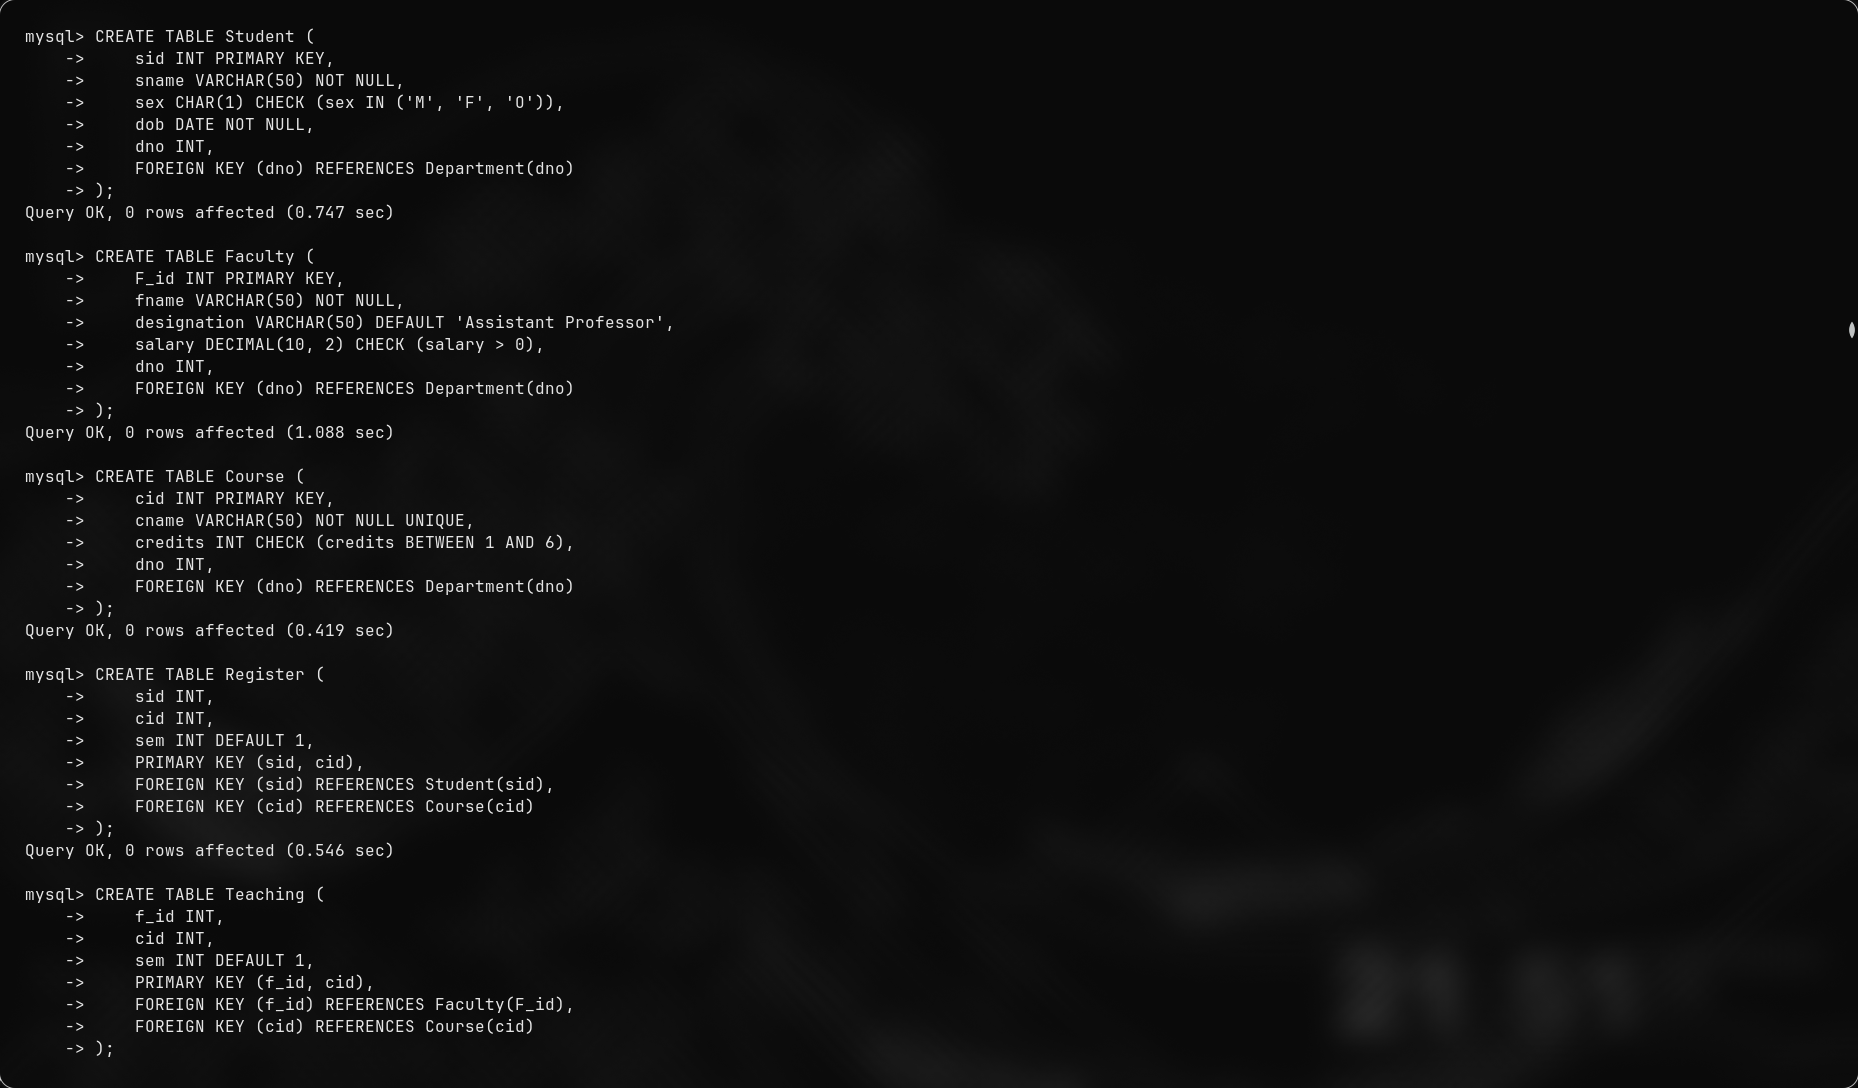
\includegraphics[width=0.92\linewidth,height=8.0cm,keepaspectratio]{Exp2-prob1-2.png}
    \caption{Creation of Student, Faculty, Course, Register, and Teaching tables with constraints.}
    \label{fig:exp2_create2}
\end{figure}

\newpage

\begin{figure}[H]
    \centering
    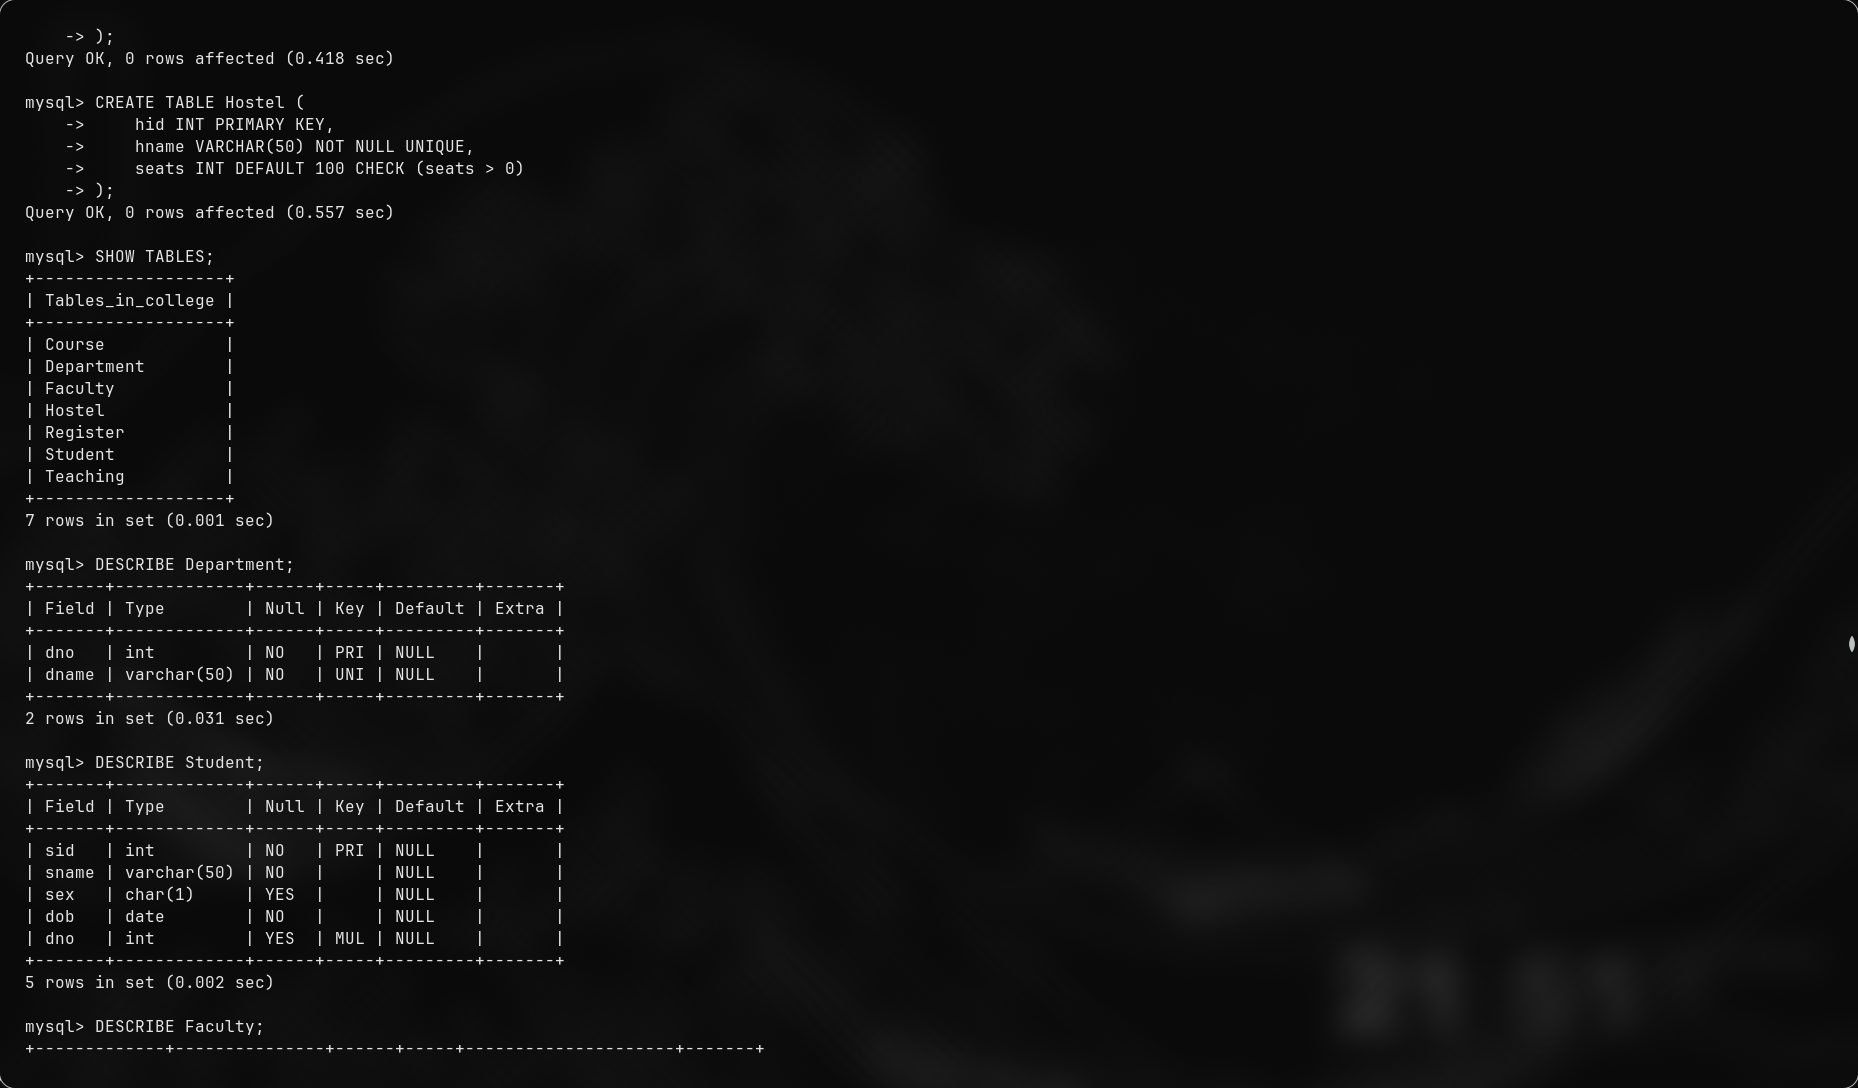
\includegraphics[width=0.92\linewidth,height=7.8cm,keepaspectratio]{Exp2-prob1-3.png}
    \caption{Hostel table creation, table catalog verification, and schema inspection of Department and Student.}
    \label{fig:exp2_inspect1}
\end{figure}

\vspace{0.2cm}

\begin{figure}[H]
    \centering
    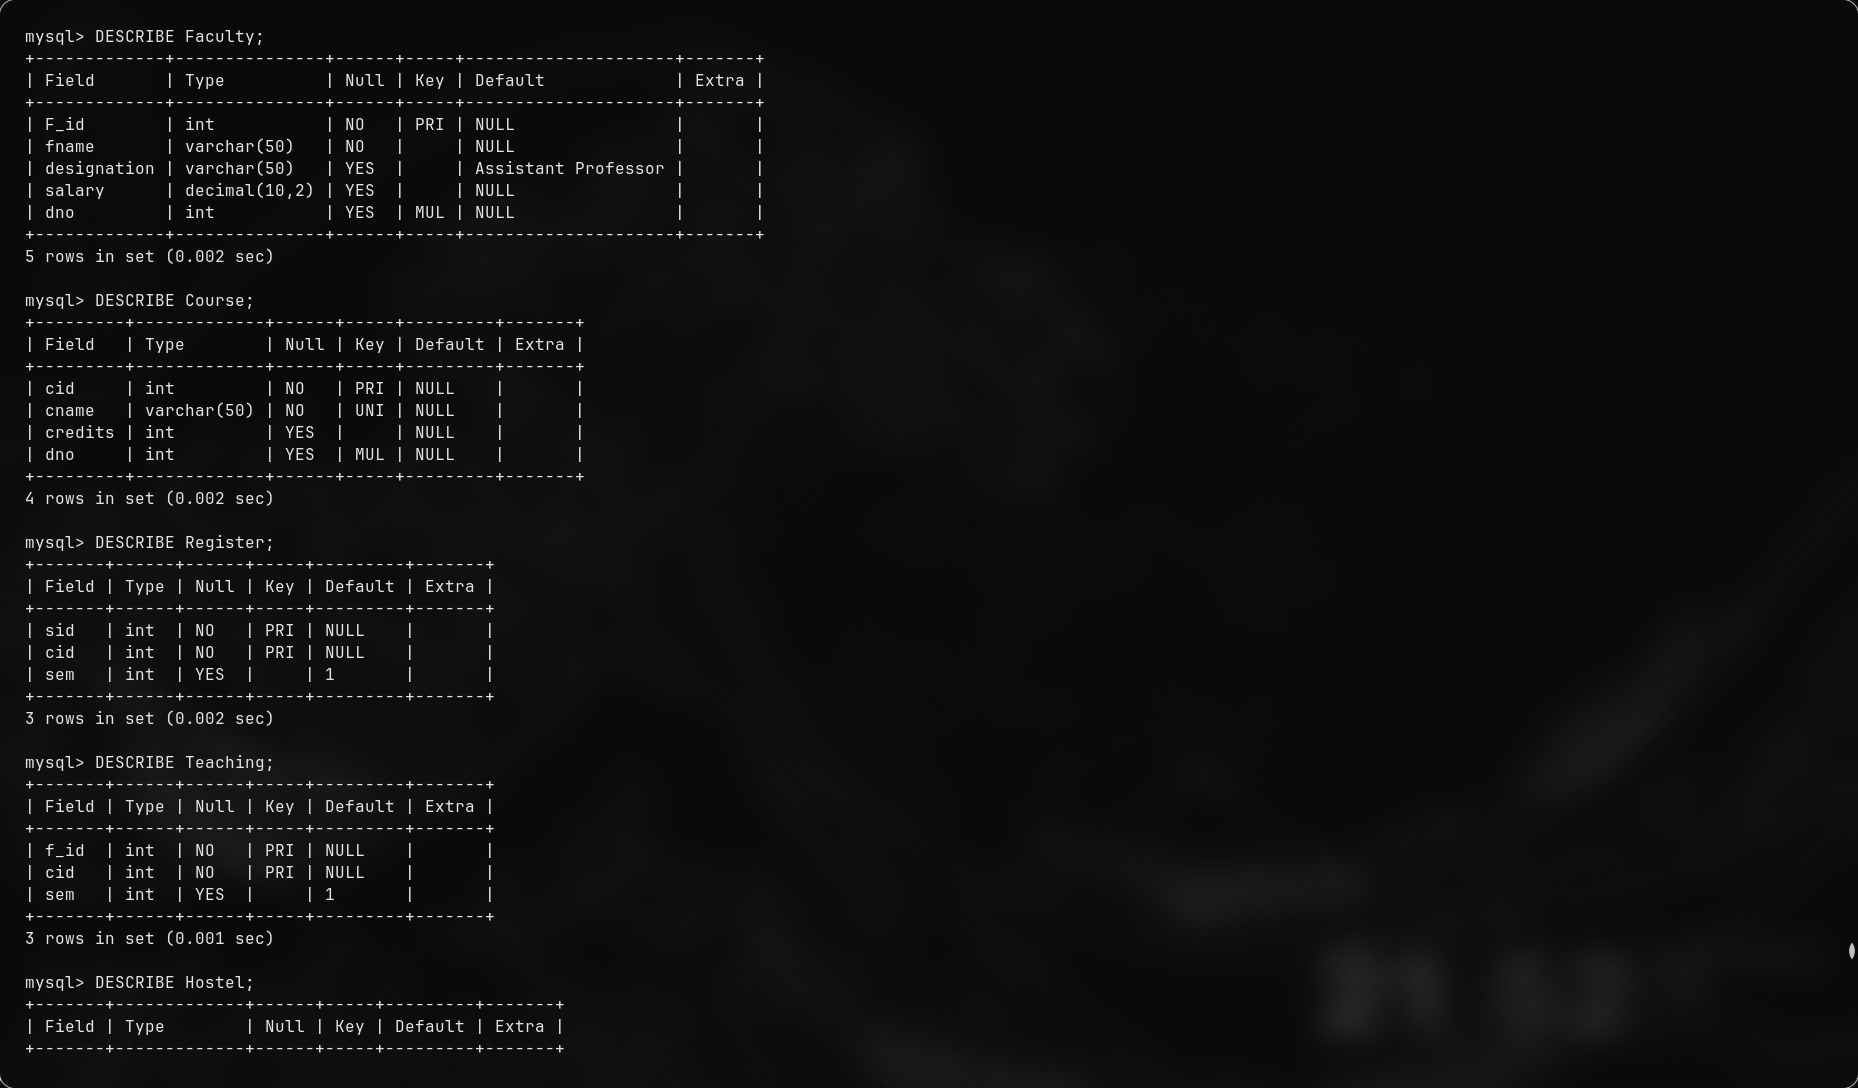
\includegraphics[width=0.92\linewidth,height=8.0cm,keepaspectratio]{Exp2-prob1-4.png}
    \caption{Schema inspection of Faculty, Course, Register, and Teaching tables.}
    \label{fig:exp2_inspect2}
\end{figure}

\newpage

\begin{figure}[H]
    \centering
    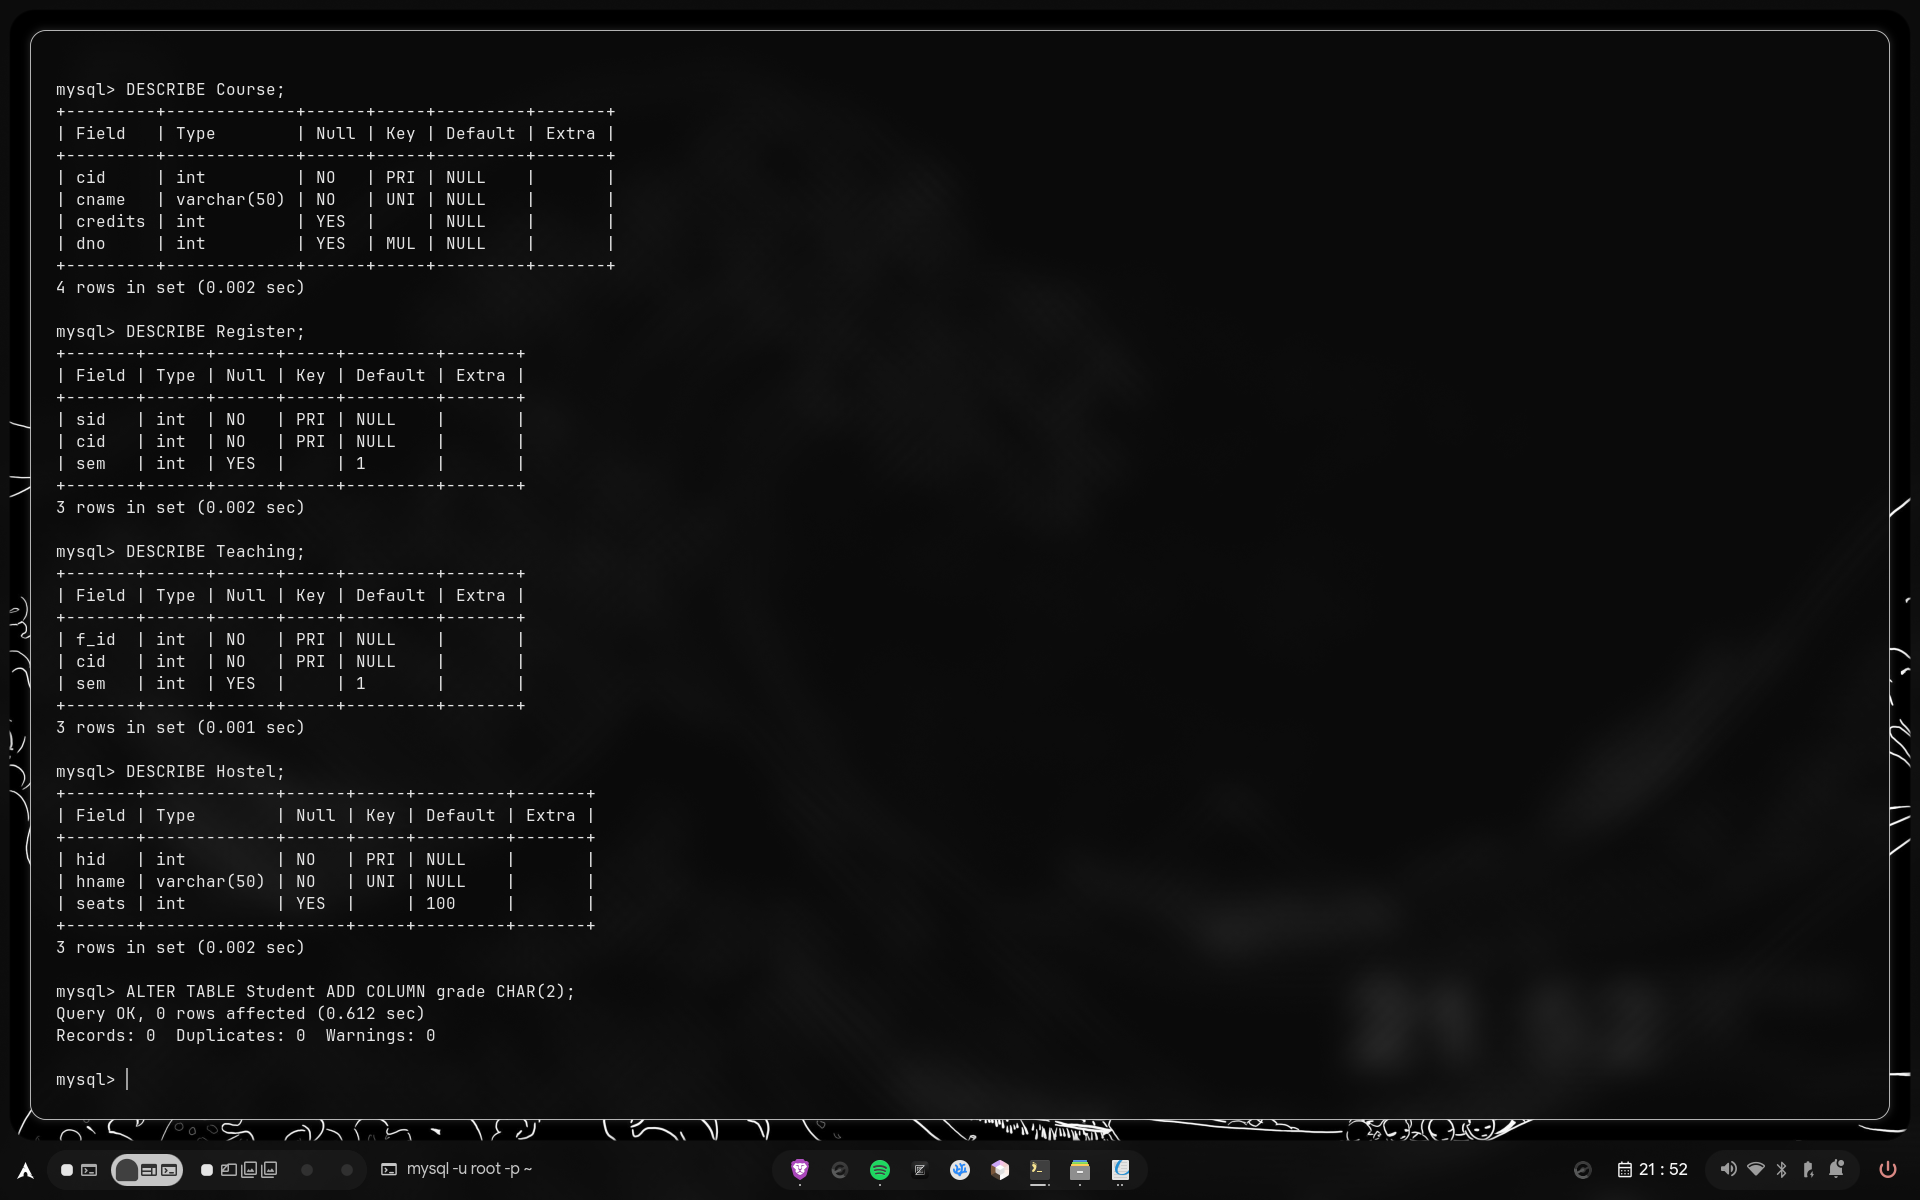
\includegraphics[width=0.92\linewidth,height=9.5cm,keepaspectratio]{Exp2-prob1-5.png}
    \caption{Hostel table schema inspection and dynamic addition of \texttt{grade} column via \texttt{ALTER TABLE}.}
    \label{fig:exp2_alter}
\end{figure}

\vspace{0.4cm}
\noindent\textbf{Result / Observation:}\quad The Data Definition Language (DDL) commands for the College database were executed successfully in MySQL. All relational tables were created with appropriate entity and referential integrity constraints, table schemas were verified via \texttt{DESCRIBE}, and structural modification using \texttt{ALTER TABLE} was confirmed.

\newpage

% =========================================================================
% EXPERIMENT 2 - PROBLEM 2: BANKING ENTERPRISE DATABASE DDL
% =========================================================================
\label{exp:ddl_prob2}
\noindent
\begin{center}
    {\LARGE \textbf{DBMS LABORATORY PRACTICAL}}\\[0.25cm]
    \textbf{Practical No.:} 2 (Problem 2) \hfill \textbf{Date:} 06/10/2026 \hfill \textbf{Page No.:} \thepage
\end{center}
\vspace{-0.2cm}
\hrule
\vspace{0.35cm}

\subsection*{Question / Problem Statement}
Consider the database for a banking enterprise. Design and implement the relational database schema using Data Definition Language (DDL) commands in MySQL:
\begin{enumerate}[noitemsep,topsep=2pt]
    \item[(i)] Create the database \texttt{bank} and select it as the active database context.
    \item[(ii)] Create the following relational tables with their integrity constraints: \texttt{customer}, \texttt{Bank\_brn}, \texttt{Deposit}, \texttt{Loan}, \texttt{Accounts\_in}, \texttt{depositor}, and \texttt{borrower}.
    \item[(iii)] Enforce primary key, foreign key, not null, check, and default constraints.
    \item[(iv)] Display all tables in the database using \texttt{SHOW TABLES;}.
    \item[(v)] Describe the schema structure of all tables using \texttt{DESCRIBE}.
    \item[(vi)] Remove the relational tables from the database using \texttt{DROP TABLE}.
\end{enumerate}

\subsection*{1. Database \& Table Creation with Integrity Constraints}

\subsubsection*{SQL Query}
\begin{lstlisting}[basicstyle=\ttfamily\footnotesize,caption={Creating bank database and relational tables with integrity constraints}]
-- Create and select bank database
CREATE DATABASE bank;
USE bank;

-- 1. customer table
CREATE TABLE customer (
    cid INT PRIMARY KEY,
    cname VARCHAR(50) NOT NULL,
    loc VARCHAR(50) NOT NULL,
    sex CHAR(1) CHECK (sex IN ('M', 'F', 'O')),
    dob DATE NOT NULL
);

-- 2. Bank_brn table
CREATE TABLE Bank_brn (
    bcode INT PRIMARY KEY,
    bloc VARCHAR(50) NOT NULL,
    bsate VARCHAR(50) NOT NULL
);

-- 3. Deposit table
CREATE TABLE Deposit (
    Dacno INT PRIMARY KEY,
    dtype VARCHAR(50) DEFAULT 'Savings',
    ddate DATE NOT NULL,
    damt DECIMAL(10, 2) CHECK (damt >= 0)
);

-- 4. Loan table
CREATE TABLE Loan (
    Lacno INT PRIMARY KEY,
    ltype VARCHAR(30) NOT NULL,
    ldate DATE NOT NULL,
    lamt DECIMAL(12, 2) CHECK (lamt > 0)
);

-- 5. Accounts_in table (composite PK, FK referencing Bank_brn and customer)
CREATE TABLE Accounts_in (
    Bcode INT,
    cid INT,
    PRIMARY KEY (Bcode, cid),
    FOREIGN KEY (Bcode) REFERENCES Bank_brn(bcode),
    FOREIGN KEY (cid) REFERENCES customer(cid)
);

-- 6. depositor table (composite PK, FK referencing customer and Deposit)
CREATE TABLE depositor (
    cid INT,
    dacno INT,
    PRIMARY KEY (cid, dacno),
    FOREIGN KEY (cid) REFERENCES customer(cid),
    FOREIGN KEY (dacno) REFERENCES Deposit(Dacno)
);

-- 7. borrower table (composite PK, FK referencing customer and Loan)
CREATE TABLE borrower (
    cid INT,
    lacno INT,
    PRIMARY KEY (cid, lacno),
    FOREIGN KEY (cid) REFERENCES customer(cid),
    FOREIGN KEY (lacno) REFERENCES Loan(Lacno)
);
\end{lstlisting}

\vspace{0.2cm}

\subsection*{2. Schema Inspection \& Table Destruction Commands}

\subsubsection*{SQL Query}
\begin{lstlisting}[basicstyle=\ttfamily\footnotesize,caption={Inspecting schema definitions and dropping tables}]
-- Display all created tables in bank database
SHOW TABLES;

-- Inspect schema definitions and constraints
DESCRIBE customer;
DESCRIBE Bank_brn;
DESCRIBE Deposit;
DESCRIBE Accounts_in;
DESCRIBE Loan;
DESCRIBE depositor;
DESCRIBE borrower;

-- Drop relational tables in referential integrity order
DROP TABLE borrower;
DROP TABLE depositor;
DROP TABLE Accounts_in;
DROP TABLE Loan;
DROP TABLE Deposit;
DROP TABLE Bank_brn;
DROP TABLE customer;
\end{lstlisting}

\newpage

\subsection*{Output Screenshots}

\begin{figure}[H]
    \centering
    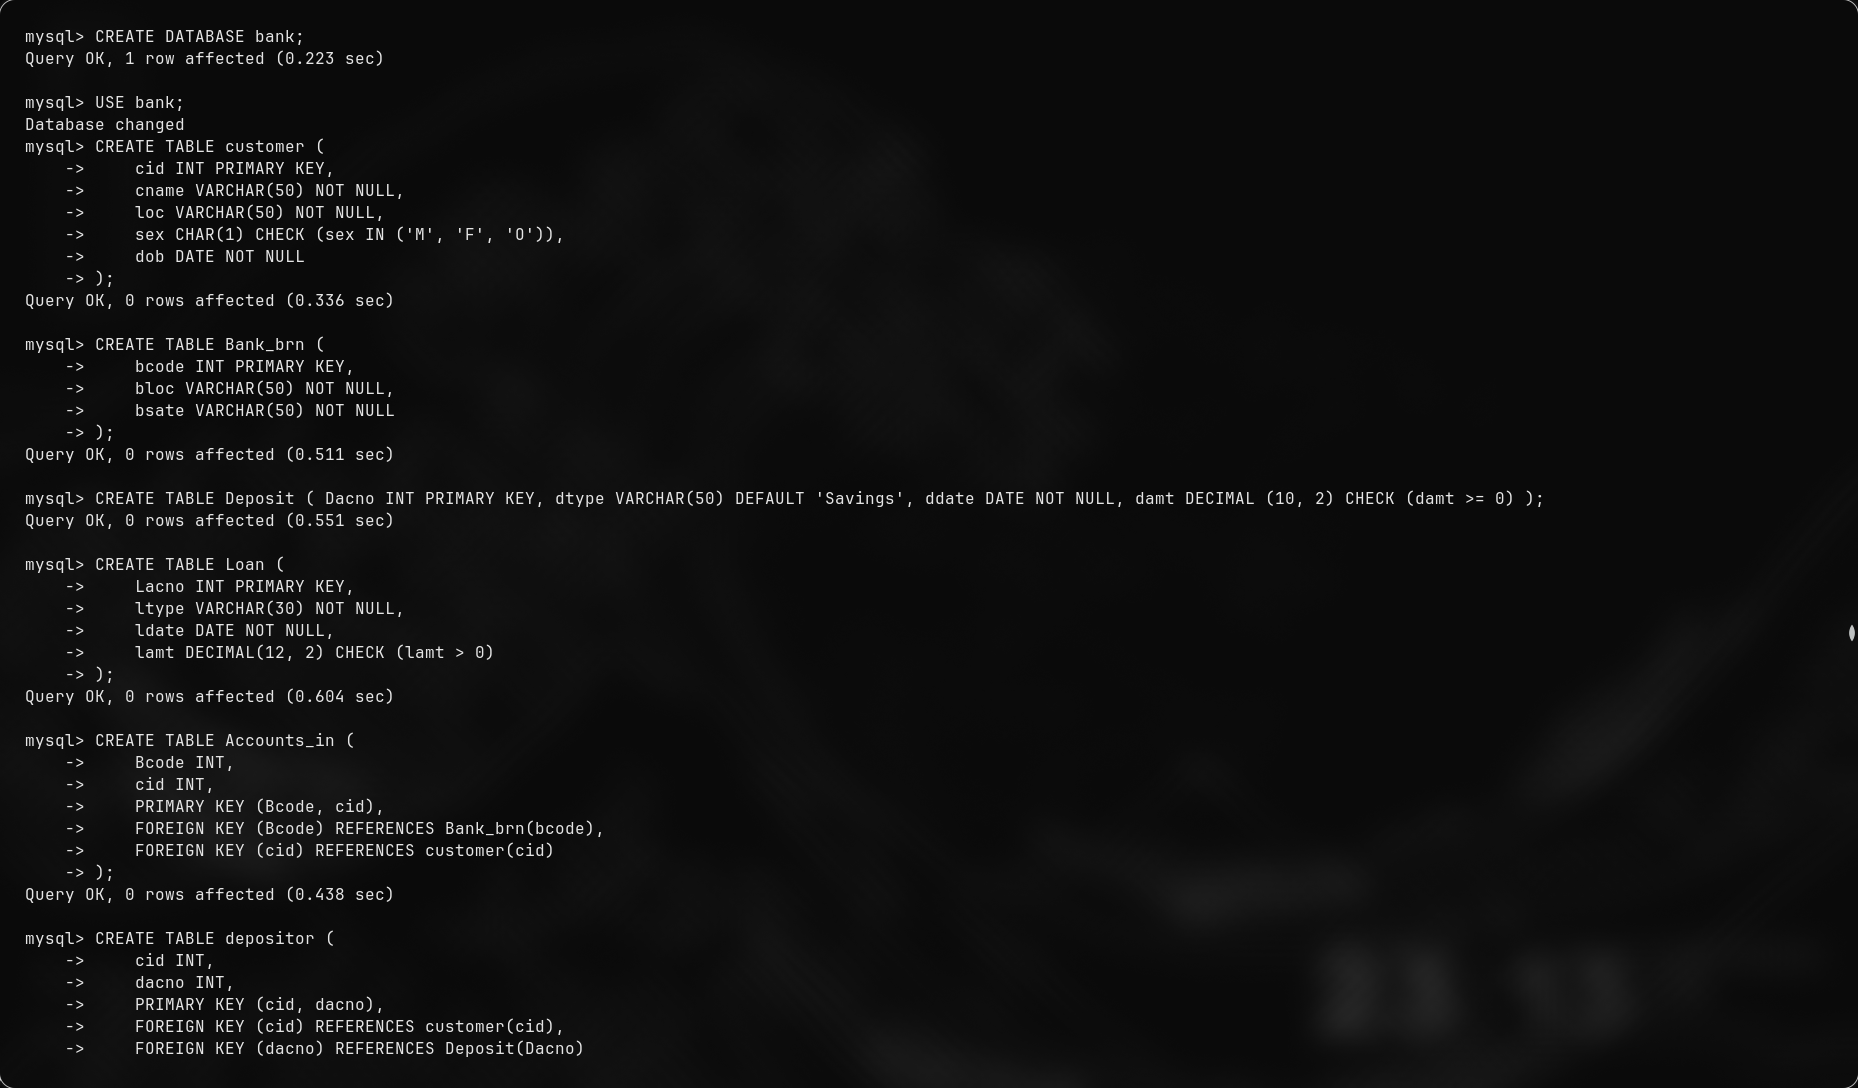
\includegraphics[width=0.92\linewidth,height=7.8cm,keepaspectratio]{Exp2-prob2-01.png}
    \caption{Database creation, active context selection, and creation of customer, Bank\_brn, Deposit, Loan, Accounts\_in.}
    \label{fig:exp2_bank_create1}
\end{figure}

\vspace{0.2cm}

\begin{figure}[H]
    \centering
    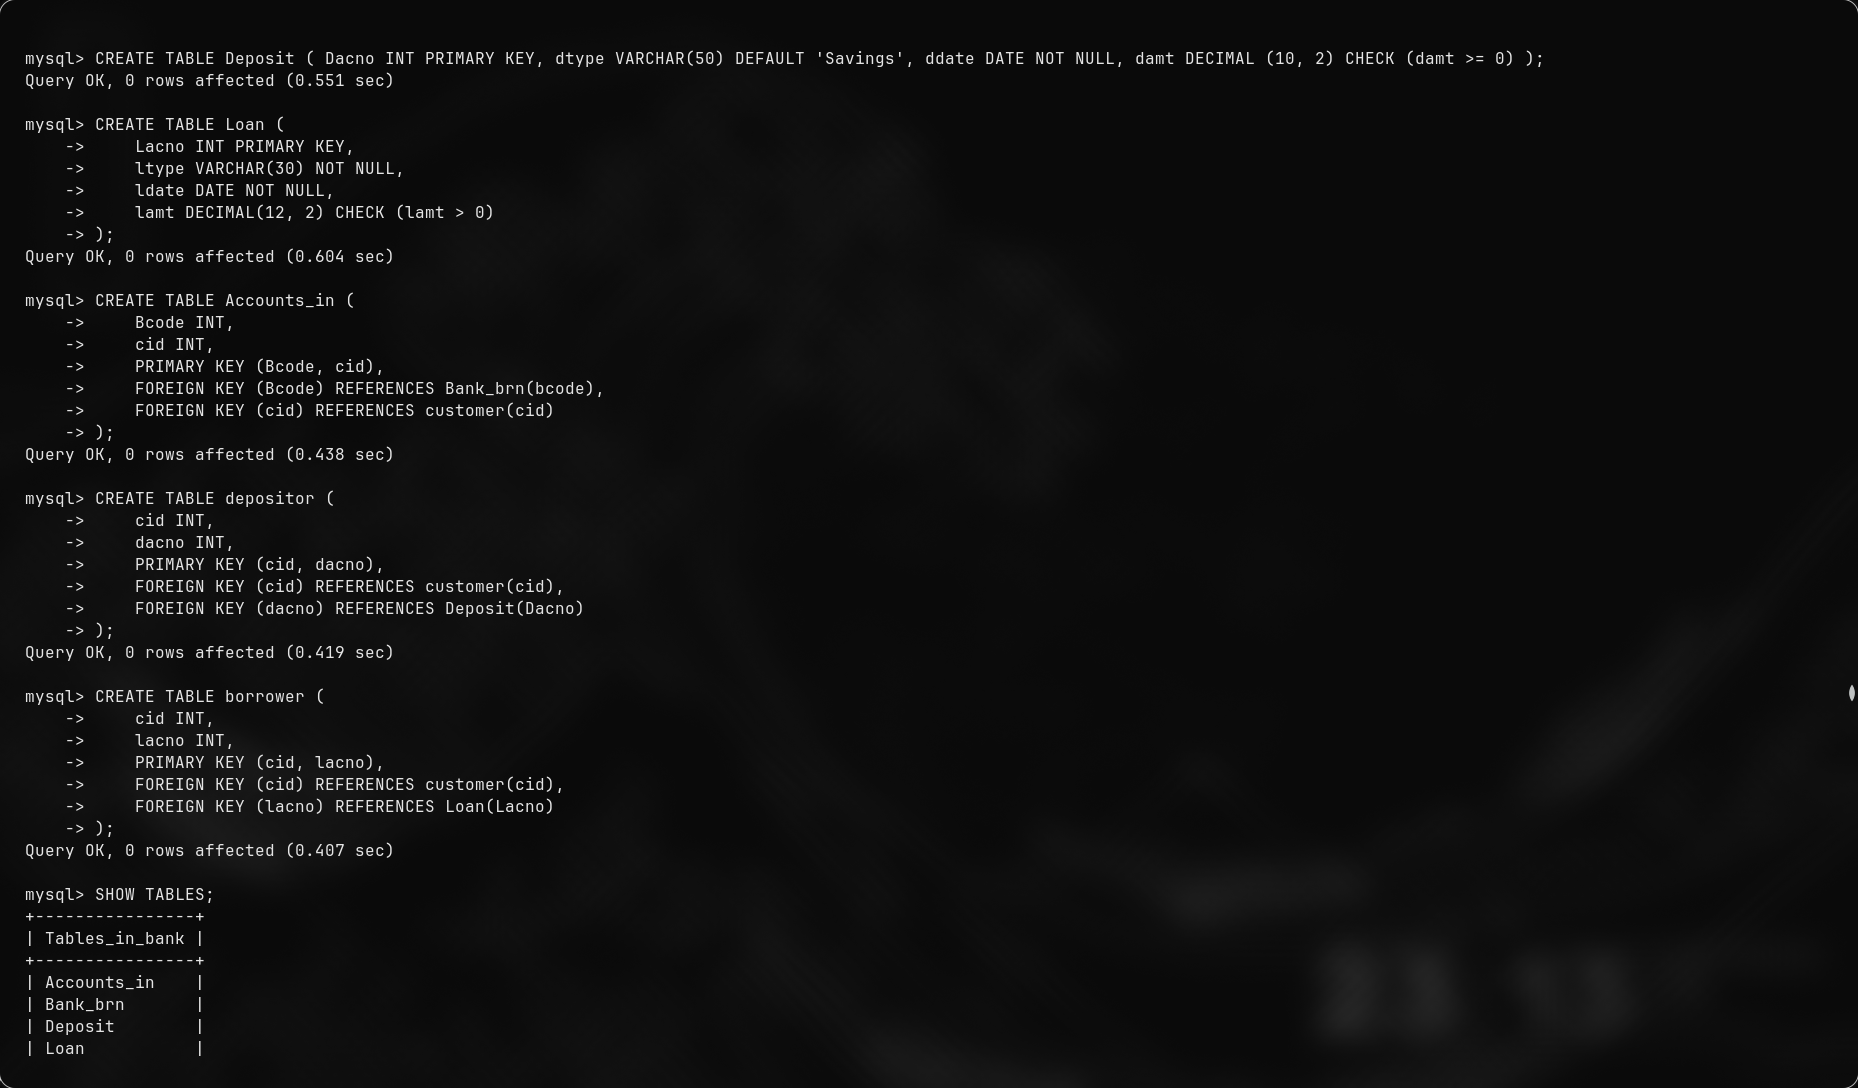
\includegraphics[width=0.92\linewidth,height=8.0cm,keepaspectratio]{Exp2-prob2-02.png}
    \caption{Creation of depositor and borrower tables with referential integrity constraints.}
    \label{fig:exp2_bank_create2}
\end{figure}

\newpage

\begin{figure}[H]
    \centering
    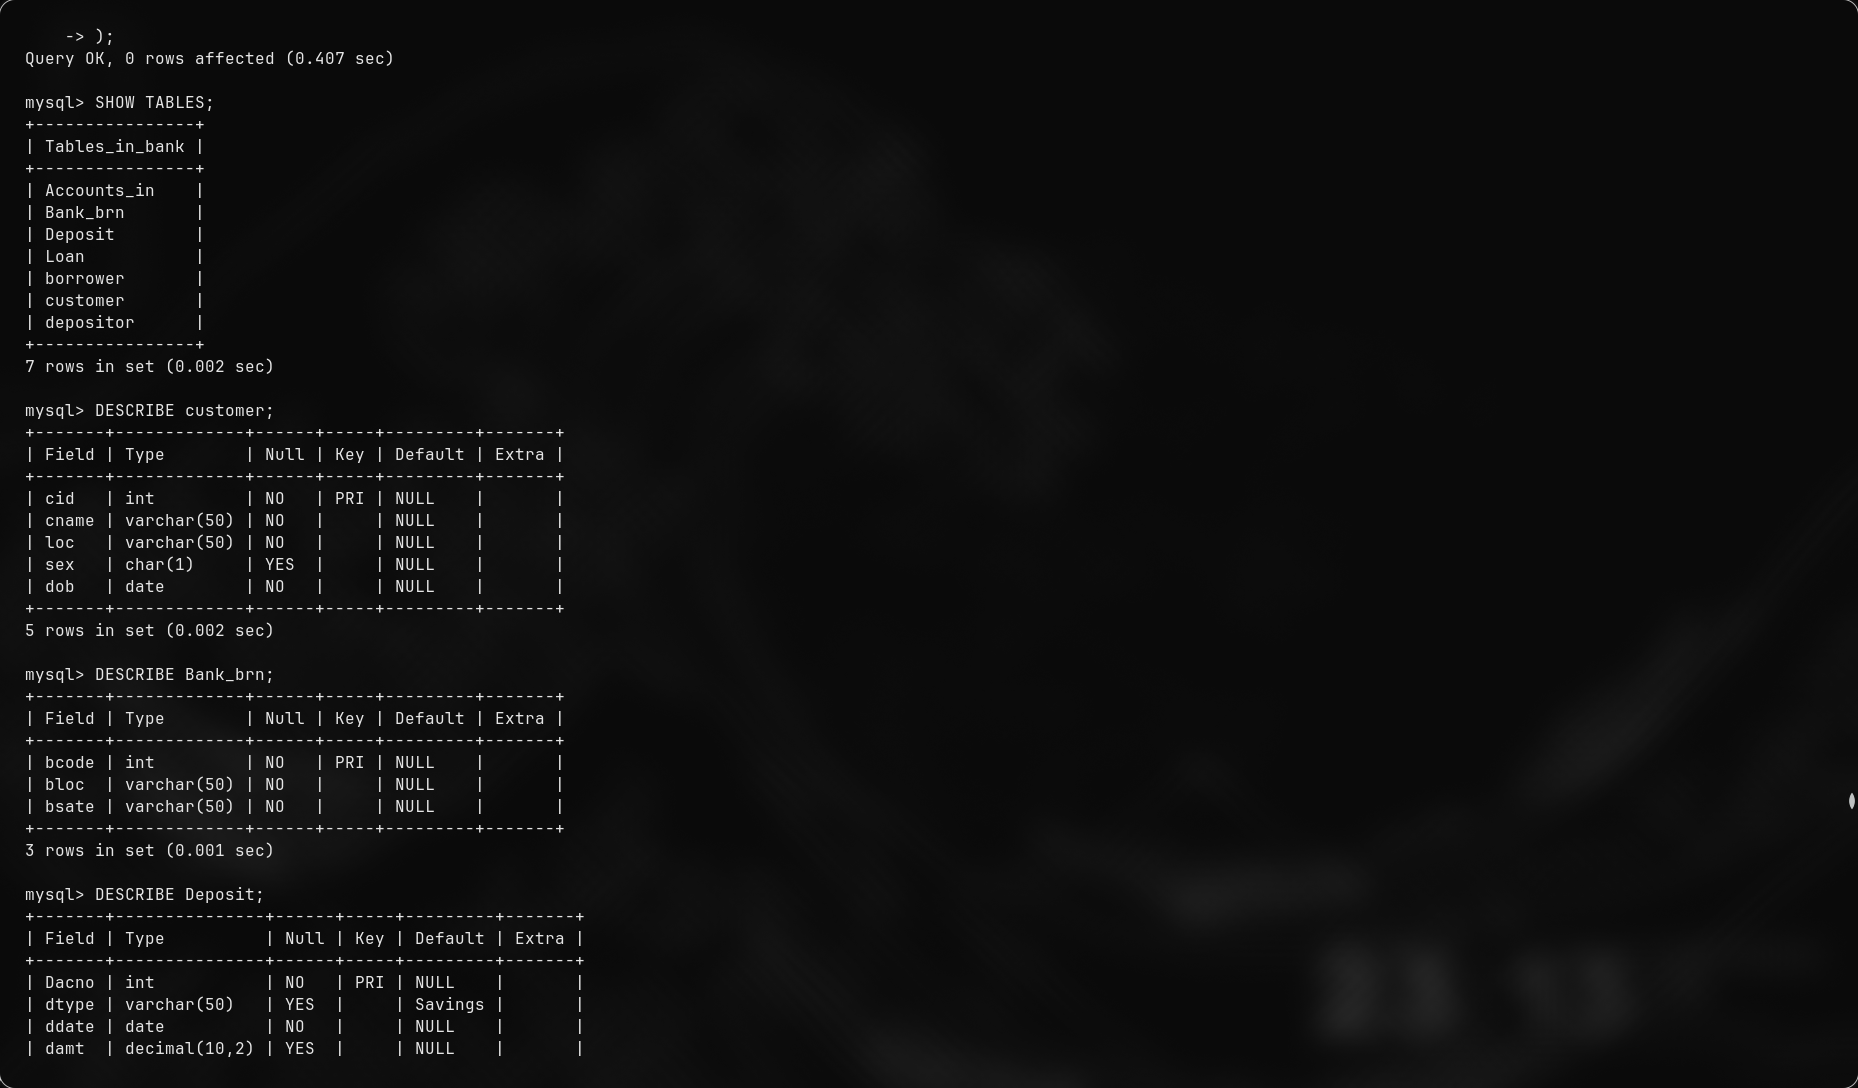
\includegraphics[width=0.92\linewidth,height=7.8cm,keepaspectratio]{Exp2-prob2-03.png}
    \caption{Verification of all seven tables via \texttt{SHOW TABLES;} and schema inspection of customer, Bank\_brn, Deposit.}
    \label{fig:exp2_bank_inspect1}
\end{figure}

\vspace{0.2cm}

\begin{figure}[H]
    \centering
    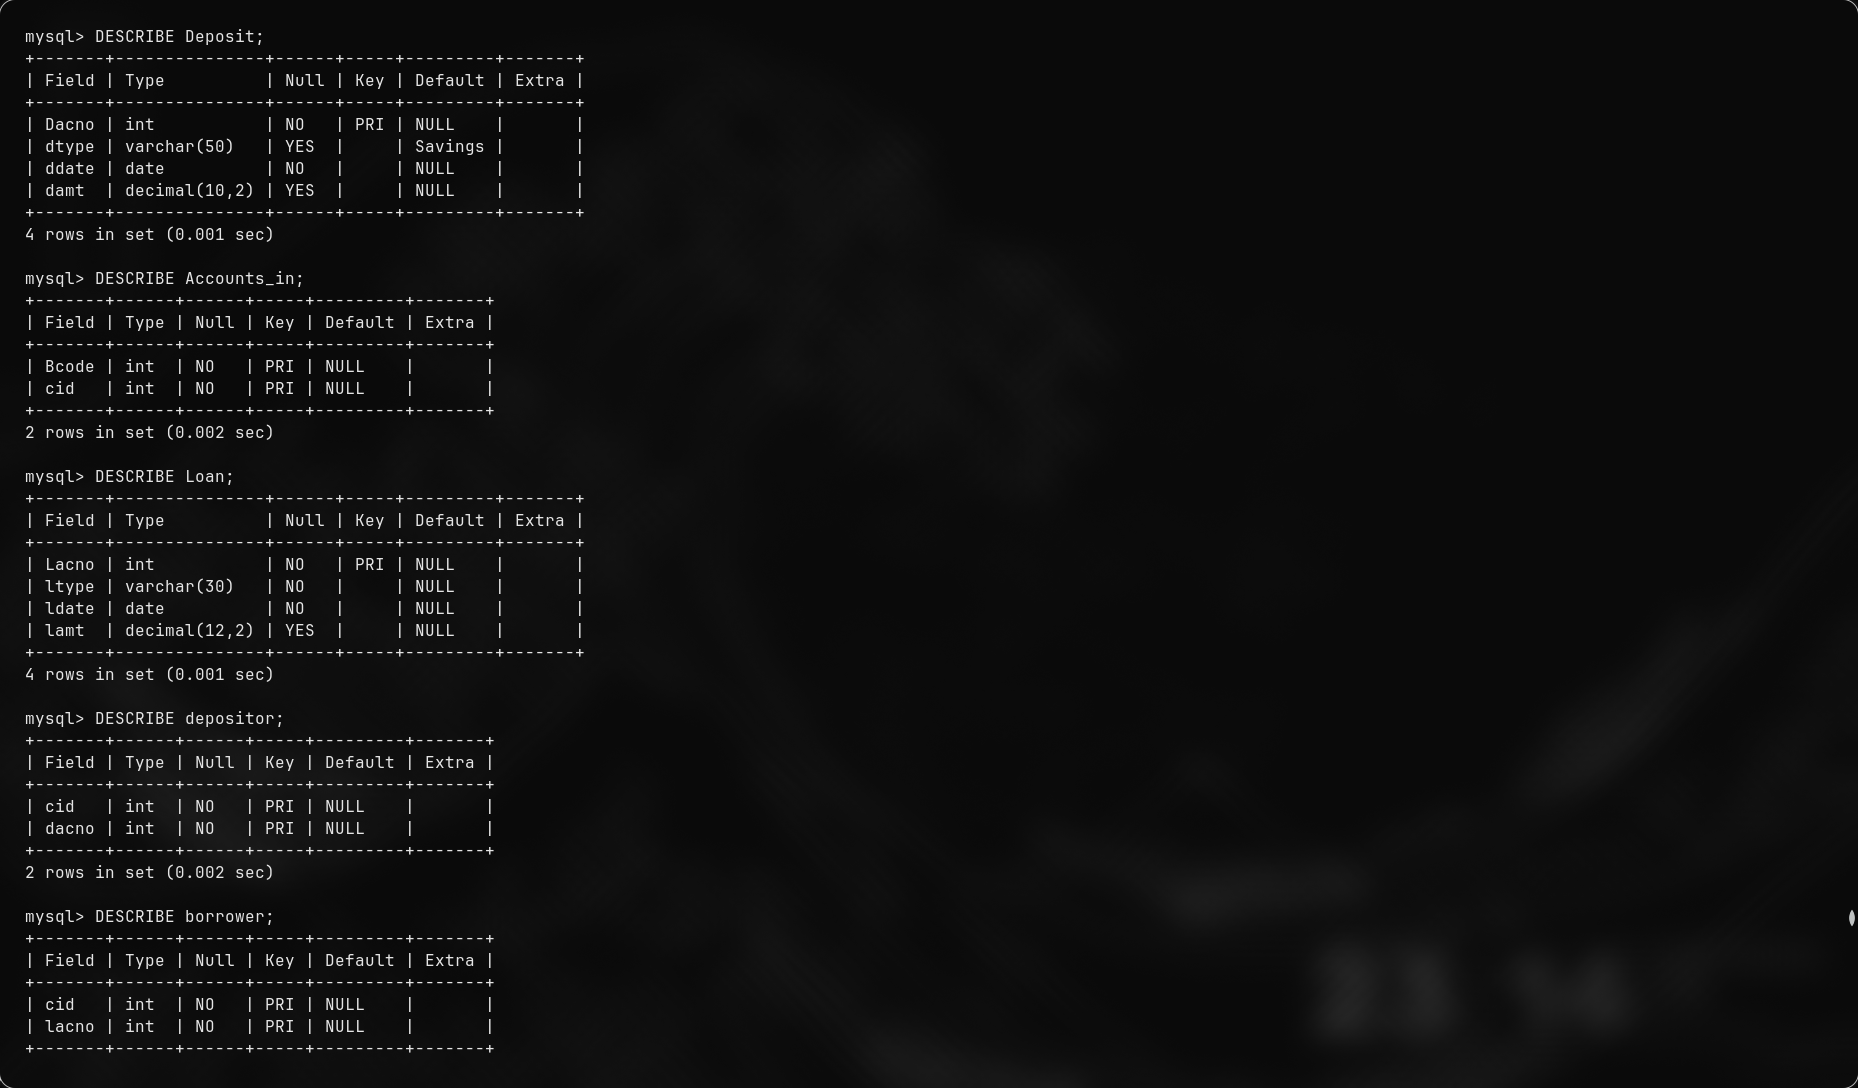
\includegraphics[width=0.92\linewidth,height=8.0cm,keepaspectratio]{Exp2-prob2-04.png}
    \caption{Schema inspection of Accounts\_in, Loan, depositor, and borrower tables.}
    \label{fig:exp2_bank_inspect2}
\end{figure}

\newpage

\begin{figure}[H]
    \centering
    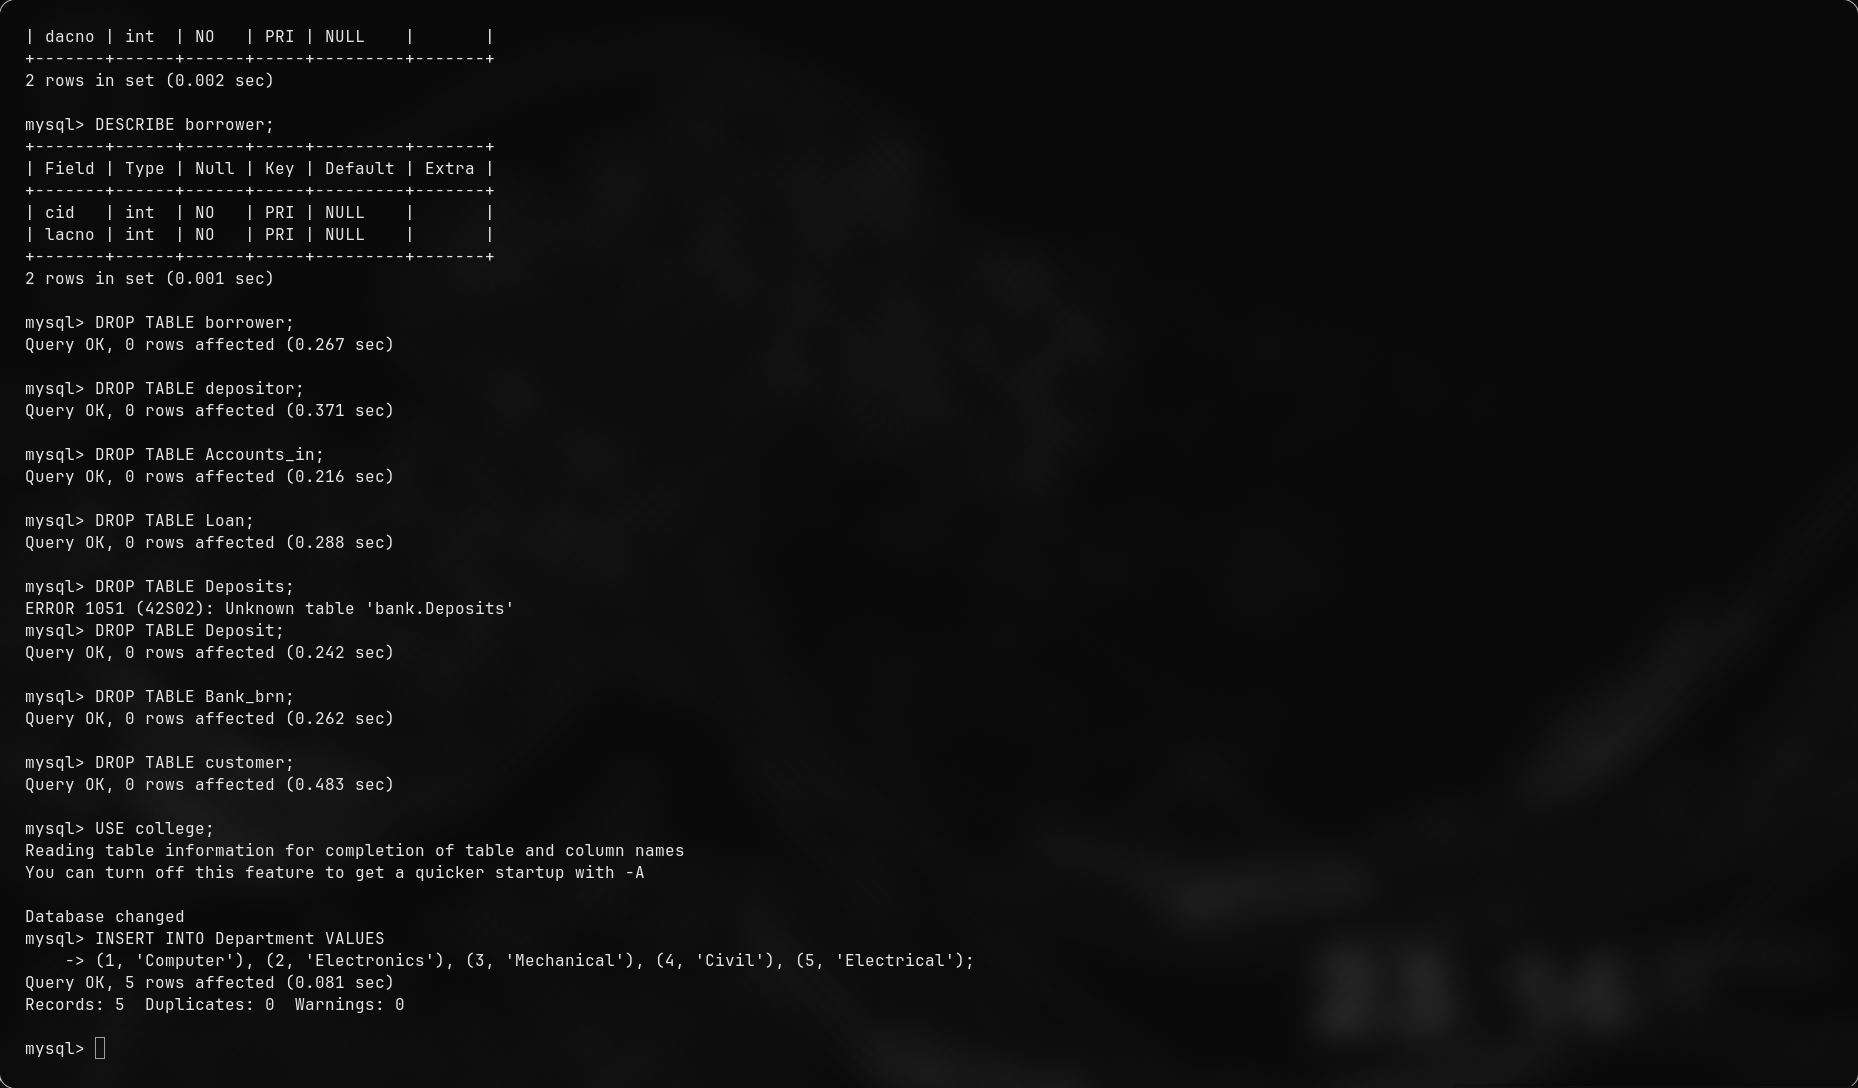
\includegraphics[width=0.92\linewidth,height=9.5cm,keepaspectratio]{Exp2-prob2-05.png}
    \caption{Final schema inspection and deletion of tables using \texttt{DROP TABLE} adhering to referential constraints.}
    \label{fig:exp2_bank_drop}
\end{figure}

\vspace{0.4cm}
\noindent\textbf{Result / Observation:}\quad The Data Definition Language (DDL) commands for the Banking Enterprise database were executed successfully in MySQL. All tables were created with proper primary key, foreign key, check, and default constraints. Schema structures were inspected via \texttt{DESCRIBE}, and tables were successfully dropped maintaining referential integrity.
